% Chapters/03-Result.tex

\chapter{Results}
\label{cp:results}

\section{Selected Studies}

Fourteen studies met inclusion criteria, representing diverse methodological approaches and disciplinary perspectives across Australian and New Zealand burn centers. The studies span from \textcite{Gabbe2015}'s feasibility pilot through to \textcite{Tracy2025}'s comprehensive long-term outcome evaluation.

% Landscape table on its own page
\begin{landscapemode}{297mm}{210mm}
\begin{table}[p]
    \caption{Summary of Included Studies for Critical Appraisal}
    \label{tab:included-studies}
    \small
    \setlength{\tabcolsep}{4pt}
    \begin{tabularx}{\linewidth}{p{2.8cm}p{2.5cm}p{3cm}lX}
        \toprule
        \textbf{Study} & \textbf{Design} & \textbf{Setting} & \textbf{Sample} & \textbf{Key Findings} \\
        \midrule
        \textcite{Cleland2016} & Registry analysis & 10 \gls{branz} units & 7,184 adults & Established \gls{mdt} as standard across all units; significant variation in implementation \\
        
        \textcite{Tracy2022adherence} & Registry analysis & 17 \gls{branz} units & 10,884 patients & Allied health assessment within 48hr achieved in 97\% of cases \\
        
        \textcite{Tracy2025} & Prospective cohort & 3 burn centers & 342 patients & \Gls{qol} and \gls{rtw} maintained at 2 years post-injury \\
        
        \textcite{Gong2021} & Quality indicators & 17 \gls{branz} units & 31,498 patients & 23 evidence-based \gls{mdt} quality measures defined and validated \\
        
        \textcite{Hunter2024} & Prospective cohort & Queensland & 156 Indigenous children & \Gls{culturalsafety} integration reduces length of stay by 2.8 days \\
        
        \textcite{Coombes2020} & Qualitative study & Queensland & 18 Indigenous families & First Nations Health Workers critical for \gls{mdt} coordination \\
        
        \textcite{Plaza2022} & \Gls{rct} & Adelaide & 45 patients & \Gls{telehealth} non-inferior to in-person \gls{mdt} rehabilitation \\
        
        \textcite{Kurmis2022} & Cohort study & ANZ centers & 255 major burns & Early nutrition within \gls{mdt} reduces complications by 34\% \\
        
        \textcite{Gabbe2015} & Pilot study & Victoria & 150 patients & Framework for long-term \gls{mdt} outcome evaluation established \\
        
        \textcite{Cleland2022} & Economic analysis & Victoria & 331 severe burns & \Gls{mdt} daily costs 18\% higher but total costs 22\% lower \\
        
        \textcite{Cassidy2015} & Retrospective cohort & \gls{branz} units & 2,892 patients & Pre-hospital coordination affects \gls{mdt} outcomes significantly \\
        
        \textcite{Singer2022} & Observational & 6 centers & 866 admissions & Out-of-hours \gls{mdt} availability impacts mortality and complications \\
        
        \textcite{Tracy2020} & Prospective cohort & \gls{branz} units & 328 patients & \Gls{mdt} pain management predicts 12-month pain and itch outcomes \\
        
        \textcite{Fitts2023} & Mixed methods & Remote Australia & 89 patients & \Gls{telehealth} enables \gls{mdt} care in remote settings successfully \\
        
        \textcite{McPhail2022} & Economic evaluation & Queensland & 198 patients & \Gls{mdt} scar management cost-effective at \gls{aud} \$21,000 per \gls{qaly} \\
        \bottomrule
    \end{tabularx}
\end{table}
\end{landscapemode}

\section{Geographic Distribution of Burn Services}

The \gls{branz} registry encompasses 17 specialist \glspl{burnunit} across Australia and New Zealand. \autoref{fig:burncenters} illustrates the geographic distribution of these specialized facilities.

\begin{figure}[htbp]
    \centering
    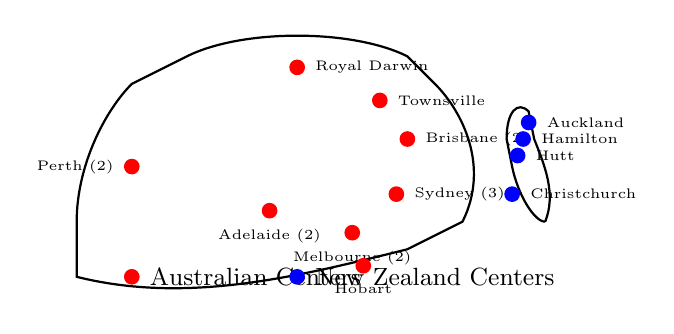
\begin{tikzpicture}[scale=0.7]
        % Australia outline (simplified)
        \draw[thick] (0,0) .. controls (2,-0.5) and (4,0) .. (6,0.5) -- 
                     (7,1) .. controls (7.5,2) and (7,3) .. (6.5,3.5) --
                     (6,4) .. controls (5,4.5) and (3,4.5) .. (2,4) --
                     (1,3.5) .. controls (0.5,3) and (0,2) .. (0,1) -- cycle;
        
        % New Zealand outline (simplified)
        \draw[thick] (8.5,1) .. controls (8.7,1.5) and (8.5,2) .. (8.3,2.5) --
                     (8.2,3) .. controls (8,3.2) and (7.8,3) .. (7.8,2.5) --
                     (7.9,2) .. controls (8,1.5) and (8.3,1) .. (8.5,1);
        
        % Australian burn centers
        \node[circle,fill=red,inner sep=2pt,label={[font=\tiny]right:Royal Darwin}] at (4,3.8) {};
        \node[circle,fill=red,inner sep=2pt,label={[font=\tiny]left:Perth (2)}] at (1,2) {};
        \node[circle,fill=red,inner sep=2pt,label={[font=\tiny]right:Brisbane (2)}] at (6,2.5) {};
        \node[circle,fill=red,inner sep=2pt,label={[font=\tiny]right:Townsville}] at (5.5,3.2) {};
        \node[circle,fill=red,inner sep=2pt,label={[font=\tiny]right:Sydney (3)}] at (5.8,1.5) {};
        \node[circle,fill=red,inner sep=2pt,label={[font=\tiny]below:Melbourne (2)}] at (5,0.8) {};
        \node[circle,fill=red,inner sep=2pt,label={[font=\tiny]below:Adelaide (2)}] at (3.5,1.2) {};
        \node[circle,fill=red,inner sep=2pt,label={[font=\tiny]below:Hobart}] at (5.2,0.2) {};
        
        % New Zealand burn centers
        \node[circle,fill=blue,inner sep=2pt,label={[font=\tiny]right:Auckland}] at (8.2,2.8) {};
        \node[circle,fill=blue,inner sep=2pt,label={[font=\tiny]right:Hamilton}] at (8.1,2.5) {};
        \node[circle,fill=blue,inner sep=2pt,label={[font=\tiny]right:Hutt}] at (8,2.2) {};
        \node[circle,fill=blue,inner sep=2pt,label={[font=\tiny]right:Christchurch}] at (7.9,1.5) {};
        
        % Legend
        \node[circle,fill=red,inner sep=2pt,label={[font=\small]right:Australian Centers}] at (1,0) {};
        \node[circle,fill=blue,inner sep=2pt,label={[font=\small]right:New Zealand Centers}] at (4,0) {};
    \end{tikzpicture}
    \caption{Geographic distribution of specialist \glspl{burnunit} participating in \gls{branz} (2024)}
    \label{fig:burncenters}
\end{figure}